\section{Group Actions and Permutations}

\begin{definition}[Symmetric Group]
    \label{def:symmetric-group}
    Let \(X\) be a set, and \(\Sym\pqty{X}\) be the set of permutations of \(X\)
    \[
        \Sym\pqty{X} = \set{\functiondomain{f}{X}{X}}{f\text{ is bijection}},
    \]
    equipped with the identity as the identity function. For \(f, g \in \Sym\pqty{X}\), we define the group operation as composition. This gives the \emph{symmetric group} of \(X\).
    
    If \(\bqty{n} = \Bqty{1, 2, \ldots, n}\), then we write \(\Sym\pqty{\bqty{n}} = S_n\).
\end{definition}

Recall from IA Groups, that it is often convenient to write \(\sigma \in S_n\) as a product of disjoint cycles. Furthermore, every \(\sigma \in S_n\) is a product of transpositions, and the number of such transpositions needed, although not fixed, has some `invariant', and is related to the \emph{sign} of \(\sigma\).

\begin{definition}[Sign of Permutation]
    \label{def:sign-of-permutation}%
    The \emph{sign} of a permutation is defined as
    \[
        \function{\sign}{S_n}{\Bqty{\pm 1}}{\sigma}{\sign\pqty{\sigma} = \begin{cases}
            1, & \sigma \text{ is a product of an even number of transpositions}, \\
            -1, & \sigma \text{ is a product of an odd number of transpositions}.
        \end{cases}}
    \]
\end{definition}

We observe that \(\sign\) is a homomorphism, and it is surjective (onto) when \(n \geq 2\).

Let \(X\) be a set and \(G\) be a group. We contemplate a homomorphism \(G \to \Sym\pqty{X}\). This is called a \emph{permutation representation} of \(G\).

\begin{definition}[Action]
    An \emph{action} of a group \(G\) on a set \(X\) is a function
    \[
        \function{\alpha}{G \times X}{X}{\pqty{g, x}}{g \ast x}
    \]
    satisfying
    \begin{itemize}
        \item \(e \ast x = x\) for all \(x \in X\);
        \item \(\pqty{g_1 \cdot g_2} \ast x = g_1 \ast \pqty{g_2 \ast x}\) for all \(g_1, g_2 \in G\) and all \(x \in X\).
    \end{itemize}
\end{definition}

We denote this as \(G \actson X\).

Now, we think of the relation between
\[
    H = \Bqty{\text{Homomorphisms } G \to \Sym\pqty{X}} \qand \Bqty{\text{Actions } G \actson X} = A.
\]

These are just sets. But we are going to define some relationship between them. Let
\[
    \function{a}{H}{A}{
        \functiondomain{f}{G}{\Sym\pqty{X}}}{
            \function{a\pqty{\phi}}{G\times X}{X}{\pqty{g, x}}{\pqty{\phi\pqty{g}}\pqty{x}.}
        }
\]

Note that \(a\pqty{\phi}\) is a group action by the homomorphism property, so this is a well-defined map.

\begin{proposition}[Bijection between Permutation Representaion and Actions]
    \label{prop:permutation-representation-actions}%
    The map \(a\) defined above is a bijection.
\end{proposition}

\begin{proof}
    We just construct an inverse map to \(a\). Let \(\functiondomain{\ast}{G \times X}{X}\) be an action. We map this to
    \[
        \function{\phi}{G}{\Sym\pqty{X}}{g}{\function{\phi\pqty{g}}{X}{X}{x}{g \ast x}.}
    \]

    We denote this as \(\phi\pqty{g} = g \ast - : X \to X\)

    Now, we claim that \(\pqty{g\inverse} \ast -: X \to X\) is the inverse, since
    \begin{align*}
        \pqty{\phi\pqty{g\inverse} \circ \phi\pqty{g}} \pqty{x} &= \phi\pqty{g\inverse} \pqty{\phi\pqty{g} \pqty{x}} \\
        &= g\inverse \ast \pqty{g \ast x} \\
        &= \pqty{g\inverse \cdot g} \ast x \\
        &= e \ast x \\
        &= x
    \end{align*}
    so \(\phi\pqty{g\inverse} \circ \phi\pqty{g} = \identity_X\).

    Similarly,
    \[
        \phi\pqty{g} \circ \phi\pqty{g\inverse} = \identity_X,
    \]
    which shows that \(\phi\pqty{g}\) is indeed \(\Sym\pqty{X}\).

    To see \(\phi\) is indeed is a homomorphism, we see
    \begin{align*}
        \phi\pqty{g_1} \circ \phi\pqty{g_2} \pqty{x} &= \phi\pqty{g_1} \pqty{\phi\pqty{g_2} \pqty{x}} \\
        &= g_1 \ast \pqty{g_2 \ast x} \\
        &= \pqty{g_1 g_2} \ast x \\
        &= \phi\pqty{g_1 g_2} \pqty{x}
    \end{align*}
    for all \(x \in X, g_1, g_2 \in G\), so we indeed have that \(\phi\pqty{g_1 g_2} = \phi\pqty{g_1} \circ \phi\pqty{g_2}\).
\end{proof}

\begin{notation}
    For an action \(G \actson X\) given by the homomorphism \(\functiondomain{\phi}{G}{\Sym\pqty{X}}\), we denote
    \begin{align*}
        G^X &= \img \pqty{\phi} \subgroup \Sym\pqty{X}, \\
        G_X &= \ker \pqty{\phi} \normalsub G.
    \end{align*}
\end{notation}

By \autoref{thm:first-isomorphism-theorem-groups} (First Isomorphism Theorem for Groups), we have
\[
    G^X \isomorphic \flatfrac{G}{G_X}.
\]

\begin{figure}[ht!]
    \centering
    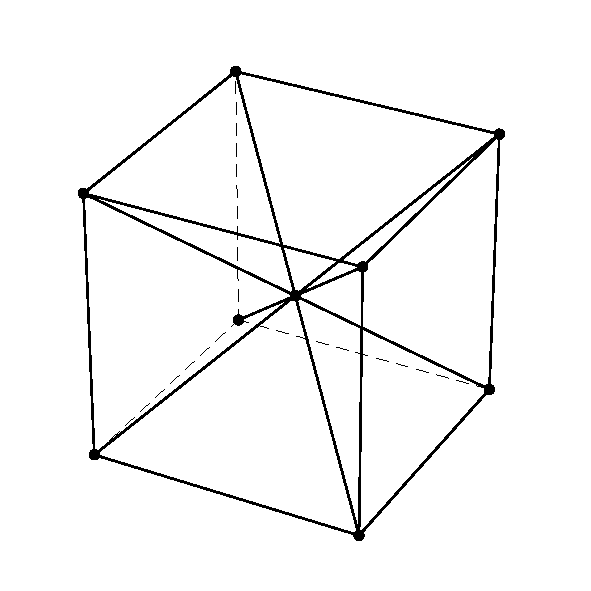
\includegraphics[scale=0.8]{fig/1-cube.pdf}
    \caption{Cube and its Diagonals}
    \label{fig:cube-diagonals}
\end{figure}

\begin{example}[Symmetry of the Cube]
    \label{ex:symmetry-of-cube}
    Let \(G\) be the symmetry group of the cube, and let \(X\) be the set of diagonals (between opposite vertices), as in \autoref{fig:cube-diagonals}. Then \(G \actson X\).

    Consider the associated  homomorphism \(\functiondomain{\phi}{G}{\Sym\pqty{X} \isomorphic S_4}\).
    
    We first show that \(\img \pqty{\phi} \isomorphic S_4\), and this can be shown by showing the transpositions lie in the image. This is trivial and left as an exercise.

    Now, consider the kernel of this map. There are two maps that keeps the diagonal unchanged: one is trivial (the identity), and one is which sends every vertex to its opposite. This means \(\ker \pqty{\phi} \isomorphic C_2\).

    Hence, we have
    \[
        \abs{G} = \abs{S_4} \cdot \abs{C_2} = 48
    \]
    by \autoref{thm:lagrange} (Lagrange's Theorem) and \autoref{thm:first-isomorphism-theorem-groups} (First Isomorphism Theorem for Groups).
\end{example}

\begin{example}[Cayley's Theorem]
    \label{ex:cayley-theorem}%
    For any group \(G\), we can write \(G\) act on (the underlying set) \(G\) by
    \[
        \function{\alpha}{G \times G}{G}{\pqty{g_1, g_2}}{g_1 g_2.}
    \]

    This induces a homomorphism \(\functiondomain{\phi}{G}{\Sym\pqty{G}}\). The kernel is
    \[
        \ker\pqty{\phi} = \set{g \in G}{g \cdot g_1 = g_1 \text{ for all }g_1 \in G} = \Bqty{e}.
    \]

    So we have \(\phi\) is injective, and hence \(G\) is some subgroup of \(\Sym\pqty{G}\) by \autoref{thm:first-isomorphism-theorem-groups} (First Isomorphism Theorem for Groups).

    This tells us that the symmetric group is \emph{very} complicated!
\end{example}

\begin{example}[Left-Multiplication on Cosets and its Kernel]
    \label{ex:left-multiplation-cosets}%
    Let \(H \subgroup G\) and \(X = \flatfrac{G}{H}\). Let \(G \actson H\) by
    \[
        \function{\alpha}{G \times \flatfrac{G}{H}}{\flatfrac{G}{H}}{\pqty{g, g_1 H}}{\pqty{g \cdot g_1} H}.
    \]

    We get the corresponding homomorphism \(\functiondomain{\phi}{G}\Sym\pqty{X}\). Trivially, we have \(\ker\pqty{\phi} \subseteq H\).

    But we have more to this. If \(g \in \ker \pqty{\phi}\), then
    \[
        g \cdot g_1 H = g_1 H
    \]
    for \emph{all} \(g_1 \in G\). Therefore,
    \[
        g_1 \inverse g g_1 \in H,
    \]
    so
    \[
        \ker\pqty{\phi} \subseteq \bigcap_{g_1 \in G} g_1 H g_1 \inverse.
    \]

    This argument is however, indeed, reversible: if
    \[
        g \in \bigcap_{g_1 \in G} g_1 H g_1 \inverse,
    \]
    then for each \(g_1 \in G\), we have
    \[
        g_1 \inverse g g_1 \in H,
    \]
    which means
    \[
        g g_1 H = g_1 H
    \]
    which means \(g \in \ker\pqty{\phi}\).

    In other words, we have
    \[
        \ker\pqty{\phi} = \bigcap_{g_1 \in G} g_1 H g_1 \inverse.
    \]

    In the special case where \(H \normalsub G\), then \(\ker\pqty{\phi} = H\). But in the general case, the right-hand side is an intersection of subgroups, which induce a normal subgroup!
\end{example}

\begin{theorem}[Normal Subgroup in Subgroup]
    \label{thm:normal-subgroup-contained-in-subgroup}%
    Let \(G\) be finite and \(H \subgroup G\) of index \(n\). Then there exists a normal subgroup \(K \normalsub G\) which also satisfies \(K \subgroup H\), such that \(\flatfrac{G}{K}\) is isomorphic to  a subgroup of \(S_n\). Thus, \(\abs{\flatfrac{G}{K}}\) divides \(n!\) and \(\abs{\flatfrac{G}{K}} \geq n\).
\end{theorem}

\begin{proof}
    Consider \(\functiondomain{\phi}{G}{\Sym\pqty{\flatfrac{G}{H}}}\) induced by the action considered in \autoref{ex:left-multiplation-cosets}. The kernel is normal in \(G\), and we let \(K = \ker \pqty{\phi}\). We have already shown it is contained in \(H\).

    By \autoref{thm:first-isomorphism-theorem-groups} (First Isomorphism Theorem for Groups), we have
    \[
        \flatfrac{G}{K} \isomorphic \img \pqty{\phi} \subgroup \Sym\pqty{\flatfrac{G}{H}} \isomorphic S_n.
    \]

    \autoref{thm:lagrange} (Lagrange's Theorem) gives \(\abs{\flatfrac{G}{H}} \divides n!\), and \(K \subgroup H\), so \(\abs{\flatfrac{G}{K}} \geq \abs{\flatfrac{G}{H}} = n\).
\end{proof}

\begin{corollary}[Non-Abelian Simple Groups]
    \label{cor:non-abelian-simple-group}%
    Let \(G\) be a non-abelian simple group. Let \(H \subgroup G\) be a proper subgroup with index \(n > 1\). Then \(G\) is isomorphic to a subgroup of \(A_n\), where \(n \geq 5\).
\end{corollary}

\begin{proof}
    We consider the same action \(G \actson \flatfrac{G}{X}\) by left-multiplication, and the homomorphism induced
    \[
        \functiondomain{\phi}{G}{\Sym\pqty{\flatfrac{G}{H}} \isomorphic S_n}.
    \]

    We look at its kernel. Since \(\ker \phi \normalsub G\), and \(G\) is simple, there are only two possibilities: \(\ker \phi = \Bqty{e}\) or \(\ker \phi = G\).

    But since \(\ker \phi \subgroup H\), and \(H\) is a proper subgroup, we have \(\ker \phi = \Bqty{e}\), so the homomorphism is injective, and by \autoref{thm:first-isomorphism-theorem-groups} (First Isomorphism Theorem for Groups),
    \[
        G \isomorphic \img \pqty{\phi} \subgroup \Sym\pqty{\flatfrac{G}{H}} \isomorphic S_n.
    \]

    For simplicity of notation, identify \(G\) with \(\img \pqty{\phi}\) and \(\Sym\pqty{\flatfrac{G}{H}}\) with \(S_n\). We know that
    \[
        G \subgroup S_n
    \]
    and we in fact want \(G \subgroup A_n\), i.e., \(G \cap A_n = G\).

    Since \(A_n \normalsub S_n\), we must have \(A_n \cap G \normalsub G\). This is by \autoref{thm:second-isomorphism-theorem-groups} (Second Isomorphism Theorem for Groups). But \(G\) is simple, so \(G \cap A_n = \Bqty{e}\), or \(G \cap A_n = G\).

    We need to rule out the case where \(G\) intersects \(A_n\) trivially. To see this, again, using \autoref{thm:second-isomorphism-theorem-groups} (Second Isomorphism Theorem for Groups), if \(G \cap A_n = \Bqty{e}\), we see that
    \[
        G \isomorphic \flatfrac{G}{G \cap A_n} \isomorphic \flatfrac{G A_n}{A_n} \leq \flatfrac{S_n}{A_n} \isomorphic C_2,
    \]
    but this is stupid since \(G\) is non-abelian.

    We last directly verify that \(S_1\) and \(S_2\) are abelian, and \(S_3\) and \(S_4\) has no non-abelian simple subgroup.
\end{proof}

\begin{definition}[Orbits, Stabalisers]
    \label{def:orbits-stablisers}%
    Let \(G \actson X\) be a group action. Let \(x \in X\).
    
    \begin{itemize}
        \item The \emph{orbit} of \(x\), denoted as \(G x\), is defined to be
        \[
            G x = \set{gx}{g \in G} \subseteq x.
        \]
        \item The \emph{stabiliser}  of \(x\), denoted as \(G_x\),is defined to be
        \[
            \set{g \in G}{gx = x} \subgroup G.
        \]
    \end{itemize}
\end{definition}

\begin{theorem}[Orbit--Stabiliser]
    \label{thm:orbit-stabiliser}%
    For \(G \actson X\) and \(x \in X\), the map \(\phi\) given as follows, is a bijection.

    \[
        \function{\phi}{Gx}{\flatfrac{G}{G_x}}{gx}{g G_x}
    \]
    
    In particular, if \(G\) is finite, we have
    \[
        \abs{G} = \abs{Gx} \cdot \abs{G_x}.
    \]
\end{theorem}